% ----------------------------------
% Diseño de contenido
% ----------------------------------


	\section{Diseño de contenido} % (fold)
	\label{sec:contenido}
	
	% section diseño_de_la_interfaz_de_usuario (end)
	\subsection{Introducción} % (fold)
		\label{sub:cont_introduccion}
	
		El diseño del contenido es una de las partes más importantes de la Usabilidad. \textbf{El motivo de que los usuarios utilicen nuestra aplicación es el contenido que les ofrezcamos.}
		
		El diseño del contenido se centra en dos tareas diferentes del diseño. En primer lugar, se desarrolla una representación del diseño para los objetos del contenido y los mecanismos requeridos para establecer una relación entre ellos. Además, se crea la información dentro de un objeto de contenido específico. El trabajo posterior consiste en generar el contenido que se usará en la \textit{webapp}.
		
		Se siguen una serie de consejos para tratar de mejorar el contenido de la aplicación:
		\paragraph{Contenido textual} % (fold)
		\label{par:cont_contenido_textual}
			\begin{itemize}
				\item \textbf{Brevedad.} Ser sucinto, es decir, solo deberemos incluir la mitad del texto que hubiéramos utilizado para escribir una publicación impresa.
				\item \textbf{Claridad.} Los usuarios no suelen detenerse mucho tiempo a leer. Por ello, se recomienda colocar la información más importante al principio, aunque sea a modo de conclusiones. Del mismo modo, tienden a leer la primera frase de cada párrafo, por lo que no es recomendable combinar ideas en un único párrafo (en muchas ocasiones, las segundas ideas pasan desapercibidas). También es recomendable evitar los textos enrevesados y utilizar con cautela el sentido del humor.
				\item \textbf{Revisión del texto.} Es muy importante revisar los textos que vamos a publicar para no cometer errores ortográficos, gramaticales, o de sintaxis que podrían perjudicar nuestra credibilidad en la aplicación.
				\item \textbf{Facultad de ojear.} Los usuarios tienden a ojear los textos deteniéndose en las palabras clave, subencabezados, etcétera. Por este motivo, resulta muy recomendable: escribir en párrafos cortos, utilizar listas numeradas o con viñetas, utilizar encabezados y subencabezados significativos y no atractivos, destacar las palabras más importantes (colores, negrita, subrayado, etcétera.).
				\item \textbf{Legibilidad.} 
			\end{itemize}
		
		% paragraph contenido_textual (end)
	
		\paragraph{Contenido gráfico y multimedia} % (fold)
		\label{par:cont_contenido_grafico_y_multimedia}
			\begin{itemize}
				\item \textbf{Tiempo de respuesta.} Muchos elementos multimedia son grandes, y su descarga lleva mucho tiempo. Por ello, siempre que se señale a un archivo que tarde más de diez segundos en descargar, es recomendable indicar el formato y el tamaño del archivo entre paréntesis tras el vínculo. Además de esto, también es recomendable incluir un avance del contenido.
				\item \textbf{Imágenes y Fotogramas.} 	Debe reducirse la cantidad de gráficos en las páginas Web. Los gráficos superfluos tiene que quitarse, dando lugar únicamente a los más relevantes para el contenido. 
				\item \textbf{Evitar imágenes tridimensionales.}
				\item \textbf{Animación y Video.} Al igual que ocurre con las imágenes, si las animaciones y los vídeos no son el eje fundamental de la página, y no son imprescindibles para comprender el contenido de la misma, deberán ser reducidos lo máximo posible. Cuando existe una imagen en movimiento, inevitablemente la atención del lector se distraerá hacia ella, de manera que dará más importancia a la misma que al propio texto. Únicamente son recomendadas para atraer la atención de los usuarios, mostrar cambios en el tiempo, en transiciones, etcétera.
			\end{itemize}

				
		% paragraph contenido_gráfico_y_multimedia (end)
	% subsection introduccion (end)
	
	
		%\begin{figure}[H]
		%  \centering
		%    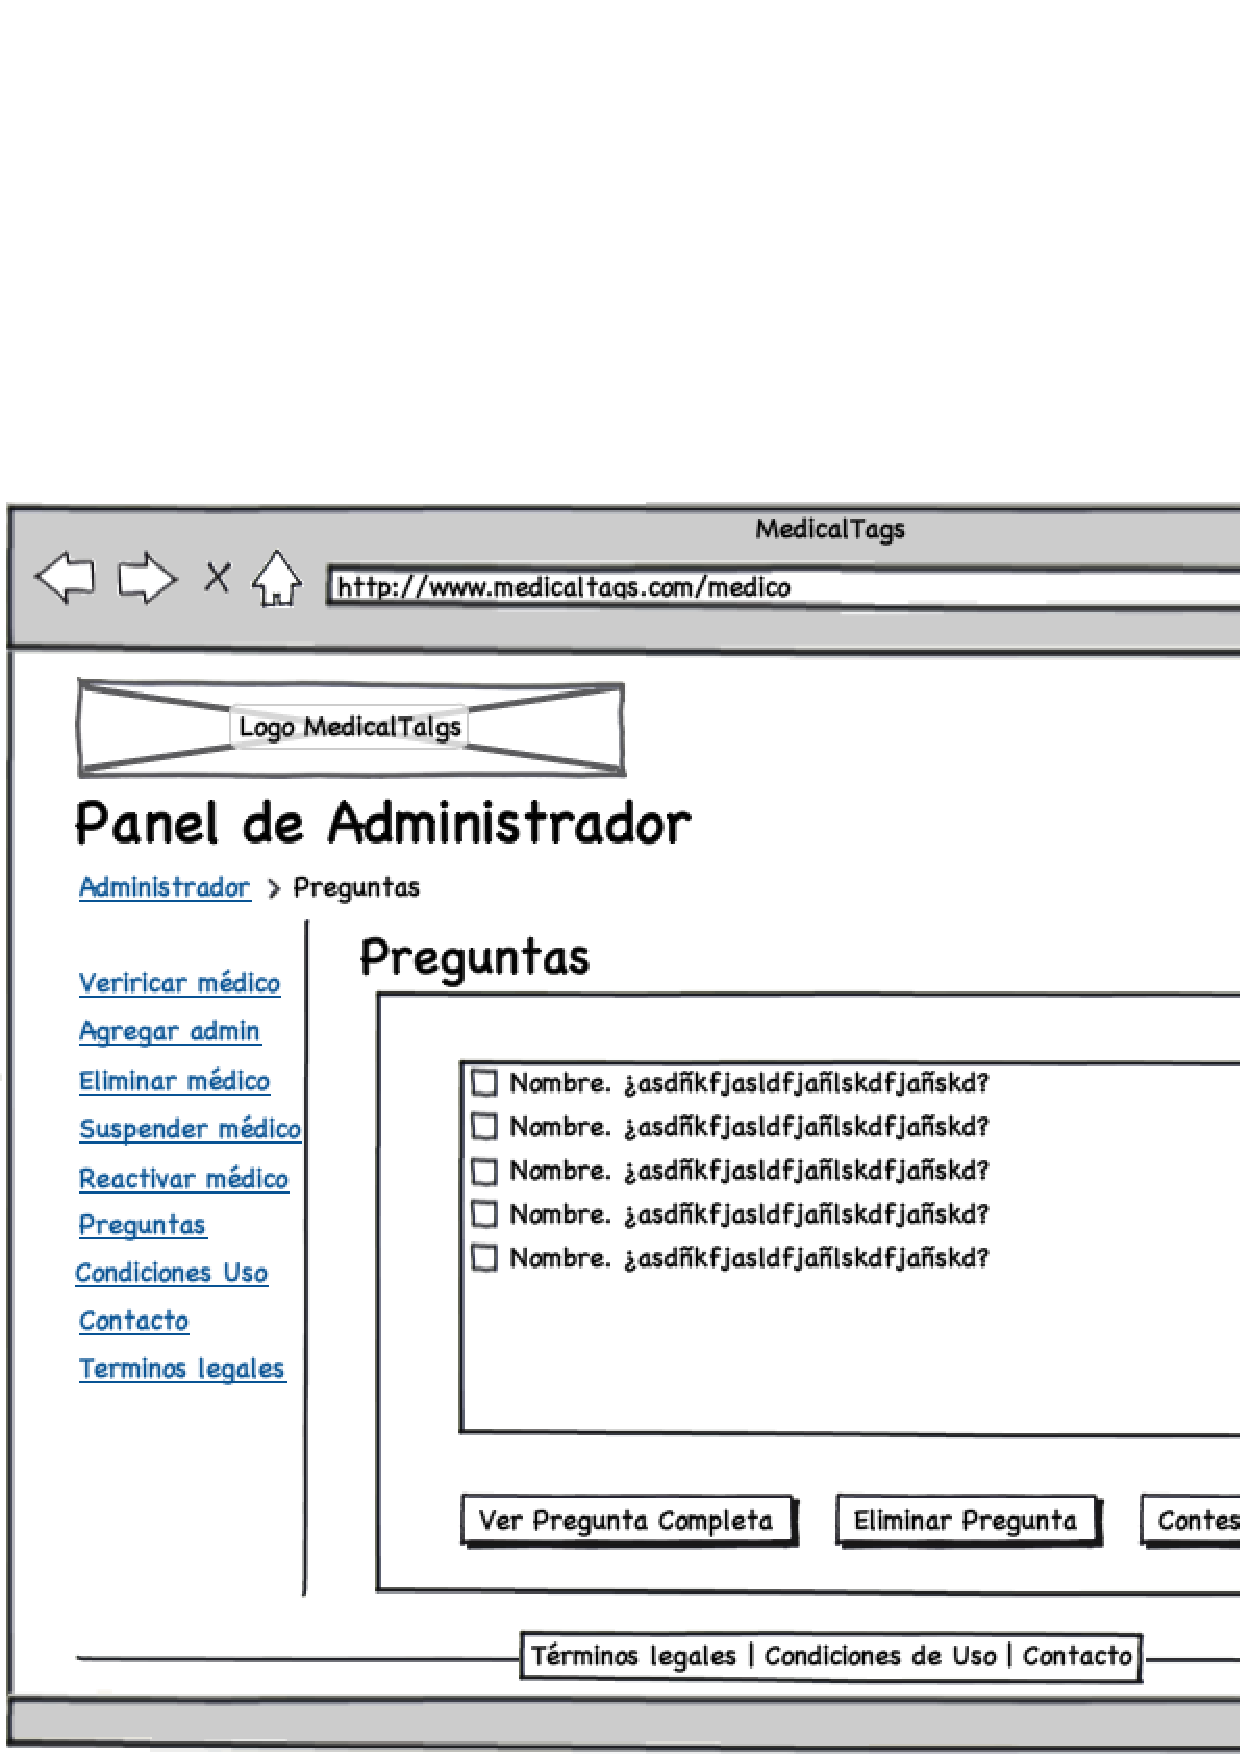
\includegraphics[width=12cm]{img/png/interfaz/99_Administrador.png}
		%  \caption{Panel de Administrador. Preguntas.}
		%  \label{fig:iu_admin_preguntas}
		%\end{figure}
	
	
	% section contenido (end)
